%\subsection{Use cases (1 p) (Jens Carl)(draft 1)}
In the process of turning the requirement specification into a fully fledged bank application, we started off developing use cases to get a better understanding about the scope of the program. Later these use cases were used as central points in the design phase. For an overview see figure \ref{fig:usecases}. Below is an example of a use case.

\subsubsection{Use case example: Performing a transaction}
\begin{itemize}
    \item[--] name: Transfer money
    \item[--] actor: customer (user)
    \item[--] main scenario: transferring money
        \begin{enumerate}
            \item User logs in.
            \item User fills out receiver field, which can either be another customer or an account id. 
            \item User selects account to transfer from.
            \item User enters amount to transfer in units of currently preferred currency.
            \item User clicks "transfer money". 
            \item Money is moved from users account.
            \item A transaction is displayed in the transaction history table. 
        \end{enumerate}
    \item[--] alternative scenario:  wrong receiver input
        \begin{enumerate}
            \item User enters a username or account id which does not exist.
            \item An error message is displayed at the top of the page. 
        \end{enumerate}
    \item[--] alternative scenario: insufficient funds
        \begin{enumerate}
            \item User enters a value larger than the amount available on their selected account. 
            \item An error message is displayed at the top of the page. 
        \end{enumerate} 
\end{itemize}
\begin{figure}[H]
    \centering 
    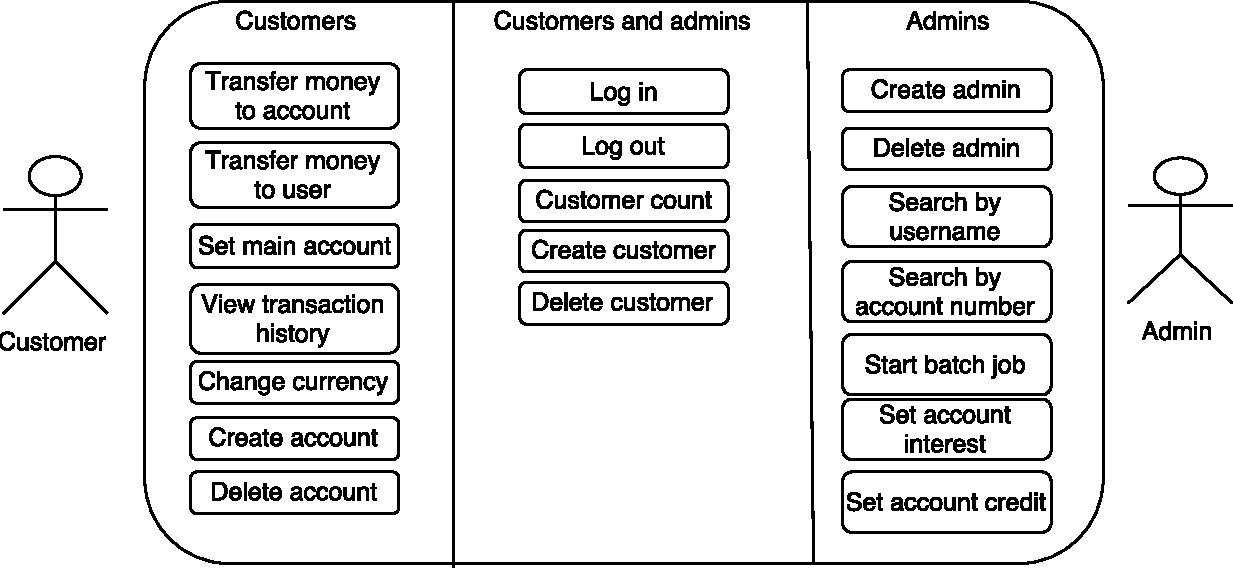
\includegraphics[width=\textwidth]{figures/use_case_diagram_final.pdf}
    \caption{Figure illustrating the different use cases. There are two different types of users; bank employees (administrators) and customers. Both users have some use cases in common, e.g. logging in and out of the application. Other cases are only preformed by one of the two. Customers need to manage their accounts and transfer money around. Admins needs to manage user profiles and account settings and perform maintenance.}
    \label{fig:usecases}
\end{figure}